\section*{گزارش شبیه‌سازی و رفع باگ کد نوشته شده در کلاس}

این قطعه کد، یک شمارنده‌ی ۴ بیتی بالا‌رونده آسنکرون (\lr{Ripple Up-Counter}) را پیاده‌سازی می‌کند که با استفاده از فلیپ‌فلاپ‌های \lr{T} ساخته شده است و می‌تواند به صورت باینری از ۰ تا ۱۵ بشمارد.

در اجرای اولیه کد، هنگام کامپایل با \lr{iverilog} با یک هشدار مواجه شدیم. از آنجا که در محیط تست‌بنچ، خروجی به صورت یک سیم تک‌بیتی (\lr{wire q;}) تعریف شده بود، کامپایلر ۳ بیت باارزش‌تر خروجی ماژول \lr{counter} را نادیده گرفت. در نتیجه، خروجی شبیه‌سازی به جای شمارش کامل، تنها لچ شدن بیت کم‌ارزش (تغییر متناوب بین ۰ و ۱) را نشان می‌داد:

\begin{latin}
    \begin{lstlisting}[basicstyle=\ttfamily\small, breaklines=true, postbreak=\mbox{\textcolor{red}{$\hookrightarrow$}\space}]
mohsen@Quanta:/mnt/D/SUT/Term_4/DSD/HW/HW-2/original$ iverilog -s Test_Bench Counter_TestBench.v
Counter_TestBench.v:38: warning: Port 2 (Q) of module counter expects 4 bit(s), given 1.
Counter_TestBench.v:38:        : Padding 3 high bits of the port.
mohsen@Quanta:/mnt/D/SUT/Term_4/DSD/HW/HW-2/original$ vvp a.out 
Time =                    0, Reset = 0, CLK = 0, Q = x
Time =                    5, Reset = 0, CLK = 1, Q = x
Time =                   10, Reset = 0, CLK = 0, Q = x
Time =                   15, Reset = 0, CLK = 1, Q = x
Time =                   17, Reset = 1, CLK = 1, Q = 0
Time =                   20, Reset = 1, CLK = 0, Q = 0
Time =                   25, Reset = 1, CLK = 1, Q = 0
Time =                   30, Reset = 1, CLK = 0, Q = 0
Time =                   35, Reset = 1, CLK = 1, Q = 0
Time =                   40, Reset = 1, CLK = 0, Q = 0
Time =                   42, Reset = 0, CLK = 0, Q = 0
Time =                   45, Reset = 0, CLK = 1, Q = 0
Time =                   50, Reset = 0, CLK = 0, Q = 1
Time =                   55, Reset = 0, CLK = 1, Q = 1
Time =                   60, Reset = 0, CLK = 0, Q = 0
Time =                   65, Reset = 0, CLK = 1, Q = 0
Time =                   70, Reset = 0, CLK = 0, Q = 1
Time =                   75, Reset = 0, CLK = 1, Q = 1
Time =                   80, Reset = 0, CLK = 0, Q = 0
Time =                   85, Reset = 0, CLK = 1, Q = 0
Time =                   90, Reset = 0, CLK = 0, Q = 1
Time =                   95, Reset = 0, CLK = 1, Q = 1
Time =                  100, Reset = 0, CLK = 0, Q = 0
Time =                  105, Reset = 0, CLK = 1, Q = 0
Time =                  110, Reset = 0, CLK = 0, Q = 1
Time =                  115, Reset = 0, CLK = 1, Q = 1
Time =                  120, Reset = 0, CLK = 0, Q = 0
Time =                  125, Reset = 0, CLK = 1, Q = 0
Time =                  130, Reset = 0, CLK = 0, Q = 1
Time =                  135, Reset = 0, CLK = 1, Q = 1
Time =                  140, Reset = 0, CLK = 0, Q = 0
Time =                  145, Reset = 0, CLK = 1, Q = 0
Time =                  150, Reset = 0, CLK = 0, Q = 1
Time =                  155, Reset = 0, CLK = 1, Q = 1
Time =                  160, Reset = 0, CLK = 0, Q = 0
Time =                  165, Reset = 0, CLK = 1, Q = 0
Time =                  170, Reset = 0, CLK = 0, Q = 1
Time =                  175, Reset = 0, CLK = 1, Q = 1
Time =                  180, Reset = 0, CLK = 0, Q = 0
Time =                  185, Reset = 0, CLK = 1, Q = 0
Time =                  190, Reset = 0, CLK = 0, Q = 1
Time =                  195, Reset = 0, CLK = 1, Q = 1
Time =                  200, Reset = 0, CLK = 0, Q = 0
Time =                  205, Reset = 0, CLK = 1, Q = 0
Time =                  210, Reset = 0, CLK = 0, Q = 1
Time =                  215, Reset = 0, CLK = 1, Q = 1
Time =                  220, Reset = 0, CLK = 0, Q = 0
Time =                  225, Reset = 0, CLK = 1, Q = 0
Time =                  226, Reset = 1, CLK = 1, Q = 0
Time =                  230, Reset = 1, CLK = 0, Q = 0
Time =                  235, Reset = 1, CLK = 1, Q = 0
Counter_TestBench.v:54: $finish called at 237 (1s)
Time =                  237, Reset = 0, CLK = 1, Q = 0
mohsen@Quanta:/mnt/D/SUT/Term_4/DSD/HW/HW-2/original$ 
\end{lstlisting}
\end{latin}

برای رفع این مشکل، تنها عرض سیم خروجی در فایل تست‌بنچ را به صورت یک باس ۴ بیتی اصلاح کردیم (\lr{wire [3:0] q;}). با اجرای مجدد کد، مشاهده می‌شود که خروجی سیستم به درستی در لبه‌های پایین‌رونده‌ی کلاک از ۰ تا ۱۵ شمرده و سپس سرریز (\lr{Overflow}) رخ می‌دهد. همچنین اعمال سیگنال‌های ریست ناهمگام نیز بلافاصله سیستم را صفر می‌کند:

\begin{latin}
    \begin{lstlisting}[basicstyle=\ttfamily\small, breaklines=true, postbreak=\mbox{\textcolor{red}{$\hookrightarrow$}\space}]
mohsen@Quanta:/mnt/D/SUT/Term_4/DSD/HW/HW-2/fixed$ iverilog -s Test_Bench Counter_TestBench_fixed.v 
mohsen@Quanta:/mnt/D/SUT/Term_4/DSD/HW/HW-2/fixed$ vvp a.out 
Time =                    0, Reset = 0, CLK = 0, Q =  x
Time =                    5, Reset = 0, CLK = 1, Q =  x
Time =                   10, Reset = 0, CLK = 0, Q =  x
Time =                   15, Reset = 0, CLK = 1, Q =  x
Time =                   17, Reset = 1, CLK = 1, Q =  0
Time =                   20, Reset = 1, CLK = 0, Q =  0
Time =                   25, Reset = 1, CLK = 1, Q =  0
Time =                   30, Reset = 1, CLK = 0, Q =  0
Time =                   35, Reset = 1, CLK = 1, Q =  0
Time =                   40, Reset = 1, CLK = 0, Q =  0
Time =                   42, Reset = 0, CLK = 0, Q =  0
Time =                   45, Reset = 0, CLK = 1, Q =  0
Time =                   50, Reset = 0, CLK = 0, Q =  1
Time =                   55, Reset = 0, CLK = 1, Q =  1
Time =                   60, Reset = 0, CLK = 0, Q =  2
Time =                   65, Reset = 0, CLK = 1, Q =  2
Time =                   70, Reset = 0, CLK = 0, Q =  3
Time =                   75, Reset = 0, CLK = 1, Q =  3
Time =                   80, Reset = 0, CLK = 0, Q =  4
Time =                   85, Reset = 0, CLK = 1, Q =  4
Time =                   90, Reset = 0, CLK = 0, Q =  5
Time =                   95, Reset = 0, CLK = 1, Q =  5
Time =                  100, Reset = 0, CLK = 0, Q =  6
Time =                  105, Reset = 0, CLK = 1, Q =  6
Time =                  110, Reset = 0, CLK = 0, Q =  7
Time =                  115, Reset = 0, CLK = 1, Q =  7
Time =                  120, Reset = 0, CLK = 0, Q =  8
Time =                  125, Reset = 0, CLK = 1, Q =  8
Time =                  130, Reset = 0, CLK = 0, Q =  9
Time =                  135, Reset = 0, CLK = 1, Q =  9
Time =                  140, Reset = 0, CLK = 0, Q = 10
Time =                  145, Reset = 0, CLK = 1, Q = 10
Time =                  150, Reset = 0, CLK = 0, Q = 11
Time =                  155, Reset = 0, CLK = 1, Q = 11
Time =                  160, Reset = 0, CLK = 0, Q = 12
Time =                  165, Reset = 0, CLK = 1, Q = 12
Time =                  170, Reset = 0, CLK = 0, Q = 13
Time =                  175, Reset = 0, CLK = 1, Q = 13
Time =                  180, Reset = 0, CLK = 0, Q = 14
Time =                  185, Reset = 0, CLK = 1, Q = 14
Time =                  190, Reset = 0, CLK = 0, Q = 15
Time =                  195, Reset = 0, CLK = 1, Q = 15
Time =                  200, Reset = 0, CLK = 0, Q =  0
Time =                  205, Reset = 0, CLK = 1, Q =  0
Time =                  210, Reset = 0, CLK = 0, Q =  1
Time =                  215, Reset = 0, CLK = 1, Q =  1
Time =                  220, Reset = 0, CLK = 0, Q =  2
Time =                  225, Reset = 0, CLK = 1, Q =  2
Time =                  226, Reset = 1, CLK = 1, Q =  0
Time =                  230, Reset = 1, CLK = 0, Q =  0
Time =                  235, Reset = 1, CLK = 1, Q =  0
Counter_TestBench_fixed.v:52: $finish called at 237 (1s)
Time =                  237, Reset = 0, CLK = 1, Q =  0
mohsen@Quanta:/mnt/D/SUT/Term_4/DSD/HW/HW-2/fixed$ 
\end{lstlisting}
\end{latin}

در نهایت، برای تایید صحت عملکرد به صورت بصری، شکل‌موج سیگنال‌ها در نرم‌افزار \lr{GTKWave} استخراج شد. در تصویر زیر به وضوح مشخص است که شمارنده با هر لبه‌ی پایین‌رونده‌ی کلاک، مقدار باس خروجی را یک واحد افزایش می‌دهد (مکث ۵۰ واحدیِ انتهای شبیه‌سازی برای خوانایی بهتر نمودار حذف شده است).

\begin{figure}[H]
    \centering
    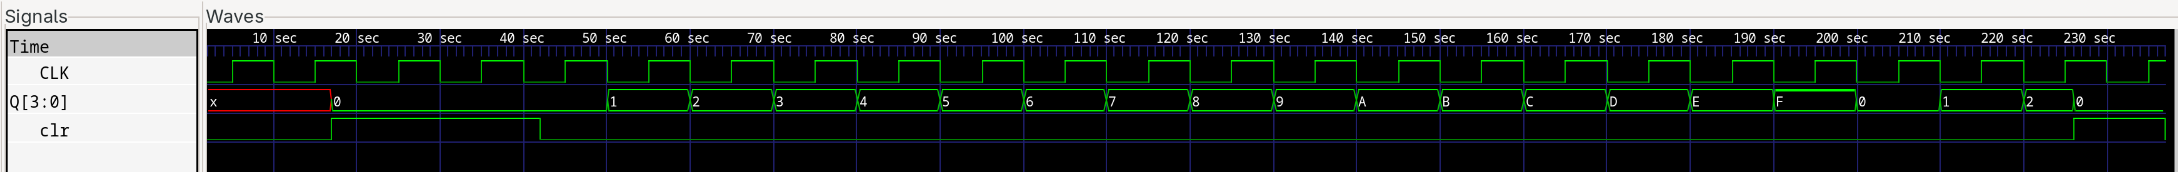
\includegraphics[width=1.0\textwidth]{assets/signal.png}
    \caption{شکل‌موج سیگنال‌های کلاک، خروجی و ریست در \lr{GTKWave}}
\end{figure}